\setchaptergraphic{}

\chapter{Differential Geometry}
\label{ch:diffgeo}

\section{Curves}

\begin{defn}
    Let $U \subseteq \R^n$ be an open set, and $f: U \to \R^m$ a function on $U$. If each component function $f^i$ has partial derivatives of all orders, we say $f$ is \emph{smooth}.
\end{defn}

\begin{defn}
    Let $U \subseteq \R^n$ and $V \subseteq \R^m$ be open sets. If $f: U \to V$ is smooth, bijective, and has a smooth inverse, then we say $f$ is a \emph{diffeomorphism}.
\end{defn}

\begin{prop}
    Given a diffeomorphism $f: U \to V$ and a point $x \in U$, the differential $df_x$ at $x$ is a linear isomorphism between $\R^n$ and $\R^m$.
\end{prop}

\begin{proof}
    We know that
    \begin{align*}
        \frac{\partial}{\partial x_i}\left(f \circ f^{-1}\right) = \left(\frac{\partial}{\partial x_i}f\right) \circ f^{-1} + f \circ \left(\frac{\partial}{\partial x_i}f^{-1}\right).
    \end{align*}
    Of course, $f \circ f^{-1}$ is the identity function, so this derivative is zero. Therefore,
    \begin{align*}
        \left(\frac{\partial}{\partial x_i}f\right) \circ f^{-1} = -f \circ \left(\frac{\partial}{\partial x_i}f^{-1}\right).
    \end{align*}
    Similarly, expanding $f^{-1} \circ f$ we get
    \begin{align*}
        \left(\frac{\partial}{\partial x_i}f^{-1}\right) \circ f = -f^{-1} \circ \left(\frac{\partial}{\partial x_i}f\right).
    \end{align*}
\end{proof}

\begin{thm}{Inverse Function Theorem}\label{thm:inverse-function}\proofbreak
    Let $S \subseteq \R^n$ be an open set, and $f: S \to \R^n$. If $df_x$ is a linear isomorphism at $x \in S$, then there exists a neighborhood $U$ of $x$ and $V$ of $f(x)$ such that $f(U) \subseteq V$ and $f: U \to V$ is a diffeomorphism.
\end{thm}

\begin{defn}
    A \emph{parameterized curve} in $\R^n$ is a map $\alpha: I \to \R^n$, where $I$ is a convex subset (interval) of $\R$.

    We say the curve is \emph{smooth} when $\alpha$ is smooth on the interior of $I$.
\end{defn}

\begin{defn}
    The \emph{trace} of a curve $\alpha: I \to \R^n$ is the image $\alpha(I)$.
\end{defn}

\begin{defn}
    A \emph{regular} curve is a smooth parameterized curve whose differential is non-zero everywhere. If $\alpha'(t) = \vec{0}$, then we say $t$ is a \emph{singular point} of the curve.
\end{defn}

\begin{figure}[ht!]
    \centering
    \begin{tikzpicture}[scale=1.0]
        \begin{axis}[
            axis x line=middle,
            axis y line=middle,
            ymin=-5,ymax=5,ylabel=$y$,
            xmin=-5,xmax=5,xlabel=$x$
            ]
        \addplot[domain=-6:6, black, ultra thick, samples=100, variable=\t] ({t^3}, {t^2});
    \end{axis}
    \end{tikzpicture}
\caption{Smooth curve with a singular point at $t = 0$, given by $\alpha(t) = (t^3, t^2)$}
\label{fig:non-regular-curve}
\end{figure}

\begin{defn}
    A curve $\alpha: I \to \R^n$ is piecewise smooth if it is continuous, and there exist a finite number of points $t_1 < t_2 < \cdots < t_k$ such that $\alpha$ is smooth when restricted to each of $(t_1, t_2), (t_2, t_3), \ldots, (t_{k-1}, t_k)$.
\end{defn}

\begin{defn}
    The \emph{arclength} of a piecewise smooth curve $\alpha: I \to \R^n$ is
    \begin{align*}
        \ell(\alpha) = \int_{I}\norm{\alpha'(s)}ds.
    \end{align*}
\end{defn}

\begin{defn}
    Let $\alpha: I \to \R^n$ and $\beta: J \to \R^n$ both be smoothed parameterized curves. We say $\beta$ is a re-parameterization of $\alpha$ if there exists a diffeomorphism $\varphi: J \to I$ such that $\beta = \alpha \circ \varphi$. Note that we then have $\alpha = \beta \circ \varphi^{-1}$, so $\alpha$ is equivalently a re-parameterization of $\beta$.
\end{defn}

\begin{prop}
    Suppose that $\alpha: (a, b) \to \R^n$ is a regular curve. Then $\psi: (a, b) \to (0, \ell(\alpha))$ given by
    \begin{align*}
        \psi(t) \mapsto \int_{a}^{t}\norm{\alpha'(s)}ds
    \end{align*}
    is a diffeomorphism.
\end{prop}

\begin{proof}
    Since $\alpha$ is regular, $\psi$ is strictly increasing and smooth, and so has a smooth inverse.
\end{proof}

\begin{defn}
    Given a regular curve $\alpha: I \to \R^n$, the map $\beta: (0, \ell(\alpha)) \to \R^n$ given by $\beta = \alpha \circ \psi^{-1}$ (where $\psi$ is as defined above) is the \emph{arclength} parameterization of $\alpha$.
\end{defn}

\begin{defn}
    A curve $\alpha: I \to \R^n$ has \emph{unit speed} if $\norm{\alpha'(t)} = 1$ for all $t \in I$.
\end{defn}

\begin{prop}
    The arclength parameterization always has unit speed.
\end{prop}

\begin{proof}
    Let $\alpha: I \to \R^n$ be a regular curve, and let $\beta: (0, \ell(\alpha)) \to \R^n$ be its arclength parameterization, where $\beta = \alpha \circ \psi^{_1}$. Then
    \begin{align*}
        \beta'(s) &= \frac{\alpha'(s)}{\psi'(s)} \\
        \norm{\beta'(s)} &= \frac{\norm{\alpha'(s)}}{\abs{\psi'(s)}} = \frac{\norm{\alpha'(s)}}{\norm{\alpha'(s)}} = 1.
    \end{align*}
\end{proof}

\begin{defn}
    The \emph{curvature} of a unit speed curve $\alpha: I \to \R^3$ is given by $\kappa(t) = \norm{\alpha''(s)}$, and the \emph{radius of curvature} is $R(s) = 1/\kappa(s)$.
\end{defn}

\begin{prop}
    The curvature of a regular curve $\alpha: I \to \R^3$ is given by
    \begin{align*}
        \kappa(s) = \frac{\norm{\alpha_{tt} \times \alpha_{t}}}{\norm{\alpha_{t}}^3}.
    \end{align*}
\end{prop}

\begin{lemma}
    Suppose $\alpha: I \to \R^n$ is a unit speed curve. Then $\alpha'': I \to \R^n$ is everywhere orthogonal to $\alpha': I \to \R^n$.
\end{lemma}

\begin{proof}
    Notice that since $\norm{\alpha'(t)} = 1$, we can differentiate to obtain
    \begin{align*}
        0 &= \alpha'(s) \cdot \alpha''(s) + \alpha''(s) \cdot \alpha'(s) = 2\alpha'(s) \cdot \alpha''(s).
    \end{align*}
\end{proof}

\begin{defn}
    If $\alpha: I \to \R^3$ is a unit speed curve with non-zero curvature at a point $s$, define $n(s)$ to be the unit vector in the direction of $\alpha''(s)$.
\end{defn}

\begin{rmk}
    Note that the tangent vector $t(s)$ has derivative $t'(s) = \alpha''(s) = \kappa(s)n(s)$.
\end{rmk}

\begin{defn}
    Let $\alpha: I \to \R^3$ be a unit speed curve whose curvature is nowhere zero. Given the tangent and normal vectors $t(s)$, $n(s)$, the plane containing the point $\alpha(s)$ and spanned by $t(s)$ and $n(s)$ is the \emph{osculating plane} at $s$.

    We then define the \emph{binormal} vector $b(s) = t(s) \times n(s)$. Note that all three of $t(s), n(s), b(s)$ are non-zero everywhere, and in fact form an orthonormal basis for $\R^3$.
\end{defn}

\begin{lemma}\label{lemma:binormal-derivative}
    Let $\alpha: I \to \R^3$ be a unit speed curve whose curvature is nowhere zero. Then $b'(s)$ is parallel to $n(s)$.
\end{lemma}

\begin{proof}
    Since $b(s) = t(s) \times n(s)$, we know
    \begin{align*}
        b'(s) = t'(s) \times n(s) + t(s) \times n'(s).
    \end{align*}
    Since $t'(s) = \kappa(s)n(s)$, it follows that $t'(s) \times n(s) = 0$, and so $b'(s)$ is normal to $t(s)$. Furthermore, $1 = b(s)^{\transpose}b(s)$, and so taking the derivative with respect to $s$ we find $b'(s)^{\transpose}b(s) = 0$. Therefore, $b'(s)$ is orthogonal to both $t(s)$ and $b(s)$, and is therefore a scalar multiple of $n(s)$.
\end{proof}

\begin{defn}
    The \emph{torsion} of a curve is $\tau: I \to \R$, such that $b'(s) = \tau(s)n(s)$.
\end{defn}

\begin{thm}{Frenet-Serret Formulas}\label{thm:frenet-serret}\proofbreak
    Let $\alpha: I \to \R^3$ be a unit speed curve whose curvature is nowhere zero. Then
    \begin{align*}
        t'(s) &= \kappa(s)n(s), \\
        n'(s) &= -\tau(s)b(s) - \kappa(s)t(s), \\
        b'(s) &= \tau(s)n(s). \\
    \end{align*}
\end{thm}

\begin{proof}
    The formula for $t'(s)$ comes directly from the definition of $n(s)$ and $\kappa(s)$, and the formula for $b'(s)$ come from Lemma \ref{lemma:binormal-derivative}. Finally,
    \begin{align*}
        n'(s) &= b'(s) \times t(s) + b(s) \times t'(s) \\
        &= \tau(s)n(s) \times t(s) + b(s) \times \kappa(s)n(s) \\
        &= -\tau(s)b(s) - \kappa(s)t(s).
    \end{align*}
\end{proof}

\begin{thm}{Fundamental Theorem of The Local Theory of Curves}\label{thm:local-theory-curves}\proofbreak
    Given functions $\kappa: I \to (0, \infty)$ and $\tau: I \to \R$, there exists a unit speed curve $\alpha: I \to \R^3$ such that $\kappa(s)$ and $\tau(s)$ are the curvature and torsion of $\alpha$ for all $s \in I$.

    Furthermore, given any two curves $\alpha: I \to \R^3$ and $\tilde{\alpha}: I \to \R^3$ with the same curvature and torsion, there exists a rigid motion such that $\tilde{\alpha}(s) = R\alpha(s) + t$ for a rotation matrix $R$ and translation $t \in \R^3$.
\end{thm}

\begin{proof}
    For existence, fix an arbitrary initial point and orthonormal basis $\langle t, n, b\rangle$, such as $\vec{0}$ and the standard basis. By the Cauchy-Lipschitz Theorem {\large\color{red}TODO} a unique solution exists.

    Given any two choices of initial conditions, there is clearly a rigid motion between. That is, if we fix a point $s_0 \in I$ then given two such curves $\alpha, \tilde{\alpha}$, let $t = \tilde{\alpha}(s_0) - \alpha(s_0)$, and let
    \begin{align*}
        R = \begin{bmatrix}
            | & | & | \\
            \tilde{t}(s_0) & \tilde{n}(s_0) & \tilde{b}(s_0) \\
            | & | & |
        \end{bmatrix}\begin{bmatrix}
            | & | & | \\
            t(s_0) & n(s_0) & b(s_0) \\
            | & | & |
        \end{bmatrix}^{-1}.
    \end{align*}
    Furthermore,
    \begin{align*}
        \frac{1}{2}\frac{d}{ds}\left(\norm{t-\tilde{t}}^2 + \norm{n-\tilde{n}}^2 + \norm{n-\tilde{n}}^2\right) &= \langle t-\tilde{t}, t' - \tilde{t'} \rangle + \langle n-\tilde{n}, n' - \tilde{n'} \rangle + \langle b-\tilde{b}, b' - \tilde{b'} \rangle \\
        &= \langle t-\tilde{t}, \kappa n - \kappa n' \rangle + \langle n-\tilde{n}, -\tau b - \kappa t - \tau \tilde{b} - \kappa \tilde{t} \rangle + \langle b-\tilde{b},\tau n - n \tilde{n} \rangle \\
        &= \kappa \langle t-\tilde{t}, n-\tilde{n}\rangle - \kappa \langle n-\tilde{n}, t-\tilde{t}\rangle - \tau\langle n-\tilde{n},b-\tilde{b}\rangle + \tau\langle b-\tilde{b}, n-\tilde{n} \rangle \\
        &= 0.
    \end{align*}
    Therefore, $t = \tilde{t}$, and so $\tilde{\alpha}(s) + t = \tilde{\alpha}$.
    {\large\color{red}TODO}
\end{proof}

\begin{defn}
    Consider a unit speed planar curve $\alpha: I \to \R^2$. The \emph{signed unit normal} $\tilde{n}$ is obtained from $t(s)$ via rotation counter-clockwise by $\pi/2$. Then the \emph{signed curvature} is $\kappa$ such that $\alpha''(s) = \kappa(s)\tilde{n}(s)$.
\end{defn}

\begin{defn}
    Let $\alpha: I \to \R^2$ be a planar unit speed curve. The \emph{signed curvature} $\kappa^{s}$ of $\alpha$ is such that $t'(s) = \kappa^{s}\tilde{n}(s)$.
\end{defn}

\begin{rmk}
    Letting $\theta(s)$ be the angle measured from the $x$-axis to $t(s)$, it follows that $t'(s) = \theta'(s)\tilde{n}(s)$.
\end{rmk}

\begin{defn}
    Given $\alpha: I \to \R^2$, where $I = (a, b)$, we can define the \emph{turning angle} $\varphi: I \to \R$ as
    \begin{align*}
        \varphi(s) = \int_{a}^{s}\kappa^{s}(\tau)d\tau.
    \end{align*}
\end{defn}

\begin{rmk}
    While $\theta(s)$ and $\varphi(s)$ are conceptually similar, they are not identical. Unlike $\theta(s)$, which may have discontinuities near the endpoints of $[0, 2\pi)$, the turning angle is continuous. Additionally, they have different initial conditions: $\varphi(0)$ is zero, while $\theta(0)$ is not generally zero.
\end{rmk}

\begin{defn}
    Let $\alpha: \R \to \R^2$ be a smooth parameterized curve. If there exists some $T > 0$ such that $\alpha(t + T) = \alpha(t$) for all $t \in \R$, we say $\alpha$ is a \emph{closed} curve. The minimum such $T$ is the \emph{period} of the curve.

    We then write $\alpha: [0, T] \to \R^2$, where $\alpha(0) = \alpha(T)$.
\end{defn}

\begin{defn}
    A \emph{Jordan curve} (or \emph{simple curve}) is a closed curve without self-intersections, i.e. if $\abs{t - s} < T$ then $\alpha(t) \neq \alpha(s)$.
\end{defn}

\begin{thm}{Sniith Schoerflies Theorem}
    Let $\alpha: [0, T] \to \R^2$ be a Jordan curve. Then there exists a diffeomorphism $f: \R^2 \to \R^2$ such that $f(S^1)$ coincides with the image of $\alpha$.
\end{thm}

\begin{rmk}
    Therefore, Jordan curves has an interior and exterior.
\end{rmk}

\begin{defn}
    Let $\alpha: [0, T] \to \R^2$ be a smooth closed curve. The \emph{turning number} of $\alpha$ is
    \begin{align*}
        I = \frac{1}{2\pi}\int_{0}^{T}\kappa^{s}ds.
    \end{align*}
\end{defn}

\begin{thm}
    Closed (but possible self-intersecting) curves always have integer turning number $I$.
\end{thm}

\begin{thm}
    Jordan curves always have turning number $I = \pm 1$.
\end{thm}

\begin{defn}
    A \emph{vertex} of a unit speed plane curve $\alpha: I \to \R^2$ is a stationary point of $\kappa^{s}$.
\end{defn}

\begin{thm}{Four Vertex Theorem}\label{thm:four-vertex-theorem}\proofbreak
    Every Jordan curve has \emph{at least} four vertices.
\end{thm}

\begin{defn}
    A Jordan curve is \emph{positively oriented} if the interior of the curve is on the left as the parameter increases.
\end{defn}

\begin{figure}[ht!]
    \centering
    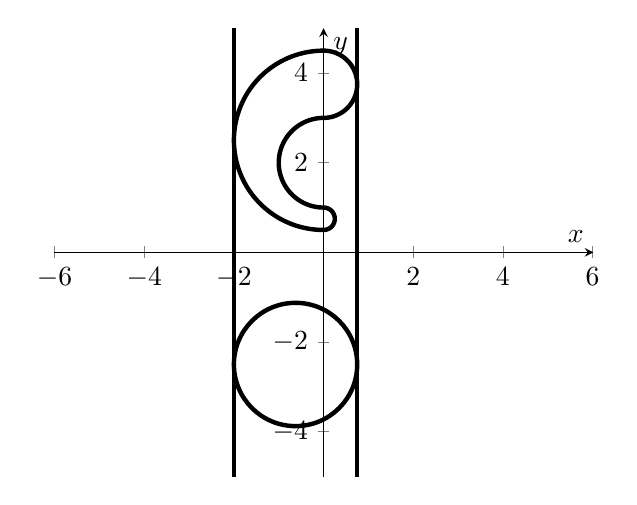
\begin{tikzpicture}[scale=1.0]
        \begin{axis}[
            axis x line=middle,
            axis y line=middle,
            axis equal,
            ymin=-5,ymax=5,ylabel=$y$,
            xmin=-5,xmax=5,xlabel=$x$
            ]
        \draw[ultra thick] (-0.625, -2.5) circle (1.375);
        \draw[ultra thick] (-2, -5) -- (-2, 5);
        \draw[ultra thick] (0.75, -5) -- (0.75, 5);

        \addplot[domain=0.25:0.75, black, ultra thick, samples=100, variable=\t] ({cos(deg(2*pi*t))}, {sin(deg(2*pi*t))+2});
        \addplot[domain=0.25:0.75, black, ultra thick, samples=100, variable=\t] ({2*cos(deg(2*pi*t))}, {2*sin(deg(2*pi*t))+2.5});
        \addplot[domain=-0.25:0.25, black, ultra thick, samples=100, variable=\t] ({0.75*cos(deg(2*pi*t))}, {0.75*sin(deg(2*pi*t))+3.75});
        \addplot[domain=-0.25:0.25, black, ultra thick, samples=100, variable=\t] ({0.25*cos(deg(2*pi*t))}, {0.25*sin(deg(2*pi*t))+0.75});
    \end{axis}
    \end{tikzpicture}
\caption{Isoperimetric inequality construction}
\label{fig:isoperimetric-construction}
\end{figure}

\begin{thm}{Isoperimetric inequality}\label{thm:isoperimetric-inequality}\proofbreak
    Among all Jordan curves $\alpha: [0, T] \to \R^2$ with the same length $T$, the circle is the unique curve attaining the maximum enclosed area.

    In particular, let $C$ be the trace of a Jordan curve with length $L$ and enclosed area $A$. Then $4\pi A \leq L^2$, with equality if and only if $C$ is a circle.
\end{thm}

\begin{proof}
    Let $v$ be an arbitary unit vector. Let $L_1$ and $L_2$ be two parallel lines, both perpendicular to $v$, and given by
    \begin{align*}
        L_1: x &= \min_{(x, y) \in C}\langle (x, y), v\rangle, \\
        L_2: x &= \max_{(x, y) \in C}\langle (x, y), v\rangle.
    \end{align*}
    Note that these maximums/minimums exist since $C$ is the continuous image of a compact set, and so is compact.

    Let $S^1$ be a circle that is tangent to both lines, and does not intersect $C$. Let $r$ be the radius of the circle, and define a coordinate system centered at $S^1$ with $y$-axis parallel to $L_1, L_2$. In this coordinate system, let $\alpha(s) = (x(s), y(s))$ be an arc-length (unit-speed) parameterization of $C$. Next, define $\tilde{y}(s) = \sqrt{r^2 - x(s)^2}$. We then define a parameterization of the circle $\tilde{\alpha}(s) = (x(s), \tilde{y}(s))$.

    Let $\tilde{A} = \pi r^2$ be the area of the circle. Using Green's Theorem, we have
    \begin{align*}
        A &= \int_{0}^{L}x(s)y'(s)ds, \\
        \tilde{A} &= -\int_{0}^{L}x'(s)\tilde{y}(s)ds.
    \end{align*}
    Therefore,
    \begin{align*}
        A + \pi r^2 &= \int_{0}^{L}xy' - x'\tilde{y}.
    \end{align*}
    By the Cauchy-Schwarz inequality,
    \begin{equation*}\tag{$\star$}\label{isoperimetric:dot-ineq}
        \abs{xy' - x'\tilde{y}} \leq \norm{\tilde{\alpha}}\norm{(y', -x')},
    \end{equation*}
    but $\norm{(y', -x')} = \norm{\alpha'} = 1$, and so
    \begin{align*}
        A + \pi r^2 \leq \int_{0}^{L}\norm{\tilde{\alpha}(t)}dt = \int_{0}^{L}rdt = rL.
    \end{align*}
    Recall that for positive $a, b$ we always have $\sqrt{ab} \leq (a + b)/2$ with equality if and only if $a = b$. Therefore,
    \begin{equation*}\tag{$\dagger$}\label{isoperimetric:area-ineq}
        \sqrt{A\pi r^2} \leq (A + \pi r^2)/2 \leq rL/2,
    \end{equation*}
    and so $A \leq L^2/(4\pi)$.

    Clearly, equality holds if $C$ is indeed a circle. It only remains to show that if equality holds, then $C$ must be a circle. For equality to hold we must have $A = \pi r^2$ in (\ref{isoperimetric:area-ineq}). Therefore, $A = L^2/(4\pi)$ gives us $L^2 = 4\pi(\pi r^2)$, and so $L = 2\pi r$. Since we could have oriented our original parallel gives $L_1, L_2$ arbitrarily by varying $v$, it must be that $C$ has constant width in all directions.

    However, just because $C$ has constant width does not mean it is a circle! For example, consider the Reuleaux triangle. However, for the equality to hold it must additionally be true that equality is attained in (\ref{isoperimetric:dot-ineq}), and so by the Cauchy-Schwarz inequality \ref{cauchy-schwarz-triangle} it follows that for all $s \in [0, L]$, there must be some $\lambda \in \R$ such that
    \begin{align*}
        \begin{pmatrix}
            x(s) \\ \tilde{y}(s)
        \end{pmatrix} &= \lambda\begin{pmatrix}
            y'(s) \\ x'(s)
        \end{pmatrix}.
    \end{align*}
    Then,
    \begin{align*}
        \lambda(s)^2 = \frac{x(s)^2 + \tilde{y}(s)^2}{x'(s)^2 + y'(s)^2} = \frac{r^2}{1}.
    \end{align*}
    In particular, $x(s) = \pm r y'(s)$. However, the parameterization of $C$ and $r$ are both independent of rotation (since $C$ is constant width), so by rotating $v$ by $pi/2$ we also have $y(s) = \pm r x'(s)$. Therefore, the curve $C$ satisfies $x^2 + y^2 = r^2y'(s)^2 + r^2x'(s)^2 = r^2$, and so is in fact a circle.
\end{proof}

\section{Surfaces}

\begin{figure}[h!]
    \centering
    \begin{minipage}[b]{0.3\linewidth}
        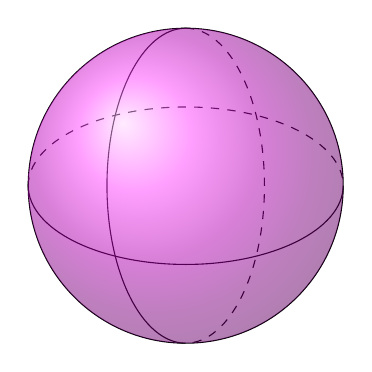
\begin{tikzpicture}
            \draw (-2,0) arc (180:360:2cm and 1cm);
            \draw[dashed] (-2,0) arc (180:0:2cm and 1cm);
            \draw (0,2) arc (90:270:1cm and 2cm);
            \draw[dashed] (0,2) arc (90:-90:1cm and 2cm);
            \draw (0,0) circle (2cm);
            \shade[ball color=Fuchsia,opacity=0.5] (0,0) circle (2cm);
        \end{tikzpicture}
    \end{minipage}
    \begin{minipage}[b]{0.3\linewidth}
        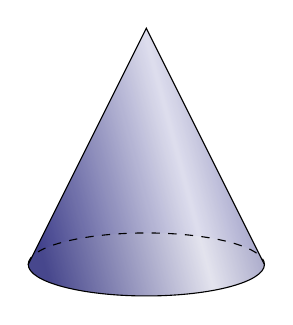
\begin{tikzpicture}
            \fill[color=blue, opacity=0.1] (-1.5,0) arc (180:0:1.5cm and 0.4cm) -- (0,3) -- cycle;
            \begin{scope}
                \path[clip] (-1.5,0) arc (180:360:1.5cm and 0.4cm) -- (0,3) -- cycle;
                \shade[left color=MidnightBlue,right color=MidnightBlue,middle color=MidnightBlue!15!white,shading angle=105,opacity=0.8] (-1.5, -1) rectangle (2.5, 3);
            \end{scope}
            \draw (-1.5,0) arc (180:360:1.5cm and 0.4cm) -- (0,3) -- cycle;
            \draw[dashed] (-1.5,0) arc (180:0:1.5cm and 0.4cm);
        \end{tikzpicture}
    \end{minipage}
    \hspace{-0.6cm}
    \begin{minipage}[b]{0.3\linewidth}
        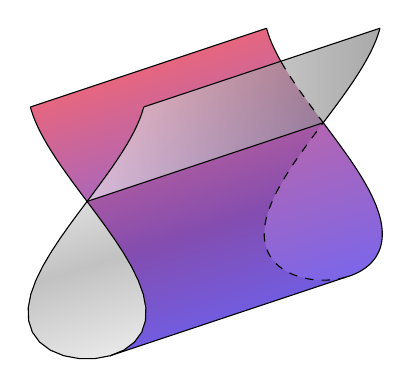
\begin{tikzpicture}[
            declare function  = {
                u(\t) = 3*\t*((\t)^2-1)/(((\t)^2+1)^2);
                v(\t) = 2*((\t)^2-1) / ((\t)^2 + 1);
            }
        ]
            \begin{scope}
                \path[clip]  plot[domain=-0.1:1] ({u(\x)}, {v(\x)}) -- plot[domain=1:-0.1] ({u(\x)+3}, {v(\x)+1}) -- cycle;
                \shade[top color=white, bottom color=white, middle color=black!60!white, shading angle=18, opacity=0.4] (-2,-2) rectangle (4,1);
            \end{scope}
            \begin{scope}
                \path[clip] plot[domain=-1:-0.1] ({u(\x)}, {v(\x)}) -- plot[domain=-0.1:-1] ({u(\x)+3}, {v(\x)+1}) -- cycle;
                \shade[top color=red!60!blue,bottom color=blue,shading angle=18,opacity=0.6] (0,-2) rectangle (4,1);
            \end{scope}
            \begin{scope}
                \path[clip] plot[domain=-1:-2] ({u(\x)}, {v(\x)}) -- plot[domain=-2:-1] ({u(\x)+3}, {v(\x)+1}) -- cycle;
                \shade[bottom color=red!30!blue,top color=red,shading angle=18,opacity=0.6] ({u(-2)},0) rectangle (3,{v(-2)+1});
            \end{scope}
            \begin{scope}
                \path[clip] plot[domain=1:2] ({u(\x)}, {v(\x)}) -- plot[domain=2:1] ({u(\x)+3}, {v(\x)+1}) -- cycle;
                \shade[left color=black!5!white,right color=black!60!white,opacity=0.6] (0,-2) rectangle (4,3);
            \end{scope}

            \draw[black] plot[domain=-2:2, samples=60] ({u(\x)+0}, {v(\x)+0});

            \draw[black] plot[domain=-2:-1.5, samples=60] ({u(\x)+3}, {v(\x)+1});
            \draw[black, dashed] plot[domain=-1.5:-1, samples=60] ({u(\x)+3}, {v(\x)+1});
            \draw[black] plot[domain=-1:-0.1, samples=60] ({u(\x)+3}, {v(\x)+1});
            \draw[black, dashed] plot[domain=-0.1:1, samples=60] ({u(\x)+3}, {v(\x)+1});
            \draw[black] plot[domain=1:2, samples=60] ({u(\x)+3}, {v(\x)+1});

            \draw[black] ({u(-2)}, {v(-2)}) -- ({u(-2)+3}, {v(-2)+1});
            \draw[black] ({u(2)}, {v(2)}) -- ({u(2)+3}, {v(2)+1});
            \draw[black] ({u(1)}, {v(1)}) -- ({u(1)+3}, {v(1)+1});
            \draw[black] ({u(-0.1)}, {v(-0.1)}) -- ({u(-0.1)+3}, {v(-0.1)+1});
        \end{tikzpicture}
    \end{minipage}
    \caption{The sphere ball and the cone (with vertex and base removed) are examples of regular surfaces, while the self-intersecting sheet is not regular surface.}
    \label{fig:diffgeom-surface-examples}
\end{figure}

\begin{defn}
    A subset $S \subseteq \R^3$ is a \emph{regular surface} if for all $p \in S$ there exists a neighborhood $W$ of $p$ (within $\R^3$), an open set $U \subseteq \R^2$, and a map $m: U \to W \intersect S$ such that
    \begin{enumerate}[label=(\roman*)]
        \item $m(u, v) = (x(u, v), y(u, v), z(u, v))$ is a smooth function,
        \item $m$ is a homeomorphism,
        \item the cross-product vector
        \begin{align*}
            \frac{\partial m}{\partial u} \times \frac{\partial m}{\partial v}
        \end{align*}
        is nowhere zero on $U$.
    \end{enumerate}
\end{defn}

\begin{rmk}\proofbreak
    \begin{enumerate}[label=(\roman*)]
        \item allows us to do calculus on surfaces,
        \item prevents self-intersection, and ensures certain properties of $S$ are independent of $W$, $U$, and $m$,
        \item ensures there is a well-defined normal vector to construct a tangent plane.
    \end{enumerate}
\end{rmk}

\begin{defn}
    A mapping $m: U \to W \intersect S$ as defined above is a \emph{local parameterization} of $S$, or a \emph{chart} for $S$. A collection of charts, such that every $p \in S$ is contained in at least one chart, is an \emph{atlas} for $S$.
\end{defn}

\begin{prop}
    The sphere $S^2$ is a regular surface. We will consider $S^2$ as a subset of $\R^3$ given by $\{p \in \R^3 : \norm{p}_2 = 1\}$.

    We will prove a chart exists for all $p \in S^2$. Consider $p \in S^2$ with positive $z$-coordinate. Take $U$ to be the open unit disc $\{u \in \R^2 : \norm{u}_2 < 1\}$, and $W$ the upper half-space $\{(x, y, z) \in \R^3 : z > 0\}$. Define the first chart $m^{(1)}: U \to W \intersect S^2$ by
    \begin{align*}
        m^{(1)}(u, v) &= \left(u, v, \sqrt{1 - (u^2 + v^2)}\right).
    \end{align*}
    This is clearly smooth since $u^2 + v^2 < 1$, and it is a homeomorphism since the inverse of $m^{(1)}$ is $(u, v, w) \mapsto (u, v)$, which is certainly continuous. Finally,
    \begin{align*}
        \frac{\partial m^{(1)}}{\partial u} \times \frac{\partial m^{(1)}}{\partial v} = \begin{pmatrix}
            1, 0, \frac{-u}{\sqrt{1 - (u^2+v^2)}}
        \end{pmatrix} \times \begin{pmatrix}
            0, 1, \frac{-v}{\sqrt{1 - (u^2+v^2)}}
        \end{pmatrix},
    \end{align*}
    which is clearly non-zero since they are linearly independent.

    We can analogously define charts for the bottom, front, top, left, right of the sphere, and so cover the entire sphere with an atlas.
\end{prop}

\begin{exmp}
    The following are examples of atlases for regular surfaces.
    \begin{itemize}
        \item A plane $\{x \in \R^3 : \langle n, x\rangle = c\}$, which can be parameterized with a single chart $m(u, v) = cn/\langle n, n \rangle + us + vt$, where $s, t$ are linearly independent vectors both perpendicular to $n$.
        \item A cut cylinder can be parameterized with the chart $m(u, v) = (a\cos(u), a\sin(u), v)$, where $U = (0, 2\pi) \times (0, 1)$.
        \item An infinite cone (without a vertex) can be parameterized with the chart
        \begin{align*}
            m(u, v) = (av\cos(u), av\sin(u), v),
        \end{align*}
        with $U = (0, 2\pi) \times (0, \infty)$.
        \item A helicoid can be parameterized by the chart $m(u, v) = (av\cos(u), av\sin(u), u)$, where $(u, v) \in (0, 2\pi) \times \R$.
        \item The sphere with a point removed can be parameterized by
        \begin{align*}
            m(u, v) = (\cos(v)\cos(u), \sin(v)\cos(u), \sin(u))
        \end{align*}
        where $(u, v) \in (-\pi/2, \pi/2) \times (0, 2\pi)$.
    \end{itemize}
\end{exmp}

\begin{prop}\label{prop:graph-is-regular-surface}
    Consider a smooth function $f: U \to \R$, where $U \subseteq \R^2$ is open. The graph of $f$ is a regular surface.
\end{prop}

\begin{proof}
    Define $m(u, v) = (u, v, f(u, v))$. Then we will show $m: U \to S$ is a chart for the graph of $f$.

    Smoothness of $m$ follows from the smoothness of $f$. The inverse of $m$ is simply the projection of $\R^3$ onto the $(u, v)$ plane, which is continuous. Finally,
    \begin{align*}
        \frac{\partial m}{\partial u} &= (1, 0, \frac{\partial f}{\partial u}), \\
        \frac{\partial m}{\partial v} &= (0, 1, \frac{\partial f}{\partial v}),
    \end{align*}
    which are trivially linearly independent.
\end{proof}

\begin{defn}
    Suppose $U \subseteq \R^n$ is open, and $F: U \to \R^m$ is smooth. We say that $p \in U$ is a \emph{critical point} of $F$ if $dF_p: \R^n \to \R^m$ fails to be surjective. If $p \in U$ is a critical point, then $F(p) \in \R^m$ is a \emph{critical value} of $F$. A point in $\R^m$ which is \emph{not} a critical value of $F$ is a \emph{regular value} of $F$.
\end{defn}

\begin{thm}
    If $f: U \to \R^3 \to \R$ is smooth, $U$ is open, and $\alpha \in f(U)$ is a regular value, then $f^{-1}(\{\alpha\})$ is a regular surface in $\R^3$.
\end{thm}

\begin{proof}
    Suppose that $p = (x_0, y_0, z_0) \in f^{-1}(\{a\})$. Since $\alpha$ is a regular value of $f$, we know $\nabla f(p) \neq \vec{0}$. Without loss of generality, we will suppose that $\frac{\partial f}{\partial z}(p) \neq 0$. Define $F: U \to \R^3$ by $(x, y, z) \mapsto (x, y, f(x, y, z))$. Then
    \begin{align*}
        dF_{p} = \begin{pmatrix}
            1 & 0 & 0 \\
            0 & 1 & 0 \\
            \frac{\partial f}{\partial x}(p) & \frac{\partial f}{\partial y}(p) & \frac{\partial f}{\partial z}(p)
        \end{pmatrix}.
    \end{align*}
    Since $\frac{\partial f}{\partial z}(p) \neq 0$ by assumption, $dF_p$ must be invertible. By the Inverse Function Theorem, there exists a neighborhood $V$ of $p$ and $W$ of $F(p)$ such that $F: V \to W$ has smooth inverse $F^{-1}: W \to V$, which necessarily has the form $F^{-1}(u, v, w) = (u, v, g(u, v, w))$ for some smooth $g: W \to \R$. Next, we can define $h: \tilde{W} \to V$ by $h(u, v) = g(u, v, \alpha)$, where $\tilde{W}$ is the projection of $W$ on to the $UV$ plane.
    
    Notice that the graph of $h$ is $f^{-1}(\{\alpha\}) \intersect V$. By Proposition \ref{prop:graph-is-regular-surface}, $h$ is a chart for $p$, and so $f^{-1}(\{\alpha\})$ must be a regular surface.
\end{proof}

\begin{cor}
    Taking $f(p) = \norm{p}_2$, we have that $S^2$ is a regular surface since $S^2 = f^{-1}(\{1\})$ and $S^2$ doesn't include $0$, which is the only critical value of $f$.
\end{cor}

\begin{thm}
    Given $S \subseteq \R^3$ be a regular surface. For any $p \in S$, there exists a neighborhood $V$ of $p$ such that $V$ is the graph of a smooth function whose form is either $z = f(x, y)$, $y = g(x, z)$, or $x = h(y, z)$.
\end{thm}

\begin{lemma}\label{lemma:change-of-chart}
    Suppose that $S$ is a regular surface and $p \in S$. Suppose that $x: U \to S$ and $y: V \to S$ are two charts of $p$. Take $\Omega = x(U) \intersect y(V)$. Then
    \begin{align*}
        h&: y^{-1}(\Omega) \to x^{-1}(\Omega), \\
        h&: (u, v) \mapsto x^{-1}(y(u, v))
    \end{align*}
    is a diffeomorphism.
\end{lemma}

\begin{proof}
    Since $x$ and $y$ are homeomorphisms by the definition of a chart, so is $h = x^{-1} \circ y$. Now fix arbitrary $r \in y^{-1}(\Omega)$, and let $q = h(r) \in x^{-1}(\Omega)$. Since $dx(q)$ and $dy(r)$ must both be injective by the third condition of the definition of a chart, it follows there is a unit vector $w$ in the orthogonal complement of the image of $dx(q)$.

    Define $F: U \times R \to \R^3$ by $F(u, v, t) = x(u, v) + tw$. Since $x$ is smooth, so is $F$. Furthermore,
    \begin{align*}
        dF(q, t) = dx(q) + tw
    \end{align*}
    must be full-rank, since $dx(q)$ is injective and $w$ is orthogonal to it's image. Therefore, we can apply the inverse function theorem \ref{thm:inverse-function} to find that $F$ is a diffeomorphism in some neighborhood $M$ of $(q, 0)$. Therefore, $h = \pi \circ F^{-1} \circ y$ (where $\pi$ is the projection on to the $uv$ plane) is smooth in a neighborhood of $r$.

    Since the roles of $x$ and $y$ are symmetric, interchanging them yields smoothness of $y^{-1} \circ x = h^{-1}$.
\end{proof}

\begin{defn}
    Let $S$ be a regular surface, and let $f: S \to \R$. Given a point $p \in S$, let $m(u, v): U \to S$ be a chart at $p$. Then $f$ is smooth at $p$ when $f \circ m$ is smooth at $m^{-1}(p)$. We say $f$ is smooth if it is smooth at all $p \in S$.
\end{defn}

\begin{lemma}
    A function $f: S \to \R$ is smooth at a point $p$, independent of the choice of chart used. That is, if it is smooth with respect to one chart then it is smooth with respect to every chart, and conversely if it is not smooth with respect to one chart then it is not smooth with repsect to any chart.
\end{lemma}

\begin{proof}
    Suppose $f: S \to \R$ is smooth at $p \in S$ with respect to a chart $x: U \to \R$, and consider another chart $y: V \to \R$, such that $p \in U \intersect V = \Omega$. But then $f \circ y = (f \circ x) \circ (x^{-1} \circ y)$. Since $f \circ x$ and $x^{-1} \circ y$ are both diffeomorphisms by assumption and by Lemma \ref{lemma:change-of-chart} respectively, $f \circ y$ must be smooth.
\end{proof}

\begin{rmk}
    We have defined the notion of a smooth function from $S \to \R$, however we can just as easily define the smoothness of a function between regular surfaces.
\end{rmk}

\begin{defn}
    Let $S_1$ and $S_2$ be regular surfaces, and consider a \emph{continuous} function $f: S_1 \to S_2$. Consider a point $p \in S_1$ and parameterizations $x: U_1 \subseteq \R^2 \to S_1$ and $y: U_2 \subseteq \R^2 \to S_2$ such that $p \in x(U_1)$ and $f(x(U_1)) \subseteq y(U_2)$. We say $f$ is smooth at $p$ if $y^{-1} \circ f \circ x: U_1 \to U_2$ is smooth at $x^{-1}(p)$.
\end{defn}

\begin{prop}
    Lemma \ref{lemma:change-of-chart} again tells us this definition is independent of the particular atlas/charts used to prove smoothness of $f$.
\end{prop}

\begin{defn}
    We say two regular surfaces $S_1$ and $S_2$ are \emph{diffeomorphic} if there exists a smooth function $f: S_1 \to S_2$ with smooth inverse.
\end{defn}

\begin{prop}
    Let $x: U \subseteq \R^2 \to S$ be a mapping satisfying the first and third conditions of the definition of a local parameterization. If $x$ is injective, then $f$ has a continuous inverse and so is a local parameterization.
\end{prop}

\begin{proof}
    {\Large\color{red}TODO: find in do Carmo}
\end{proof}

\section{Tangent planes and differentials}

\begin{defn}
    Let $S \subseteq \R^3$ be a regular surface. A vector $v$ is a \emph{tangent vector} to $p \in S$ if there exists a smooth curve $\alpha: (-\varepsilon, \varepsilon) \to S$ such that $\alpha(0) = p$ and $\alpha'(0) = v$.
\end{defn}

\begin{defn}
    Let $S \subseteq \R^3$ be a regular surface, and $p \in S$. The \emph{tangent plane} of $S$ at $p$ is the set of tangent vectors to $S$ passing through $p$, and is denoted by $T_pS$.
\end{defn}

\begin{prop}
    Let $x: U \to S$ be a local parameterization of a regular surface $S$, and let $q \in U$. Then $dx_q$ is a linear isomorphism between vectors in $\R^2$ and the tangent plane at $p$.
\end{prop}

\begin{proof}
    Let $w$ be a tangent vector to $S$ at $x(q)$, so $w = \alpha'(0)$ for some smooth curve $\alpha: (-\varepsilon, \varepsilon) \to S$, with $\alpha(0) = x(q)$. In particular, for $\varepsilon$ small enough, $x$ is a local parameterization for all points in the trace of $\alpha$. Therefore, we consider the curve $\beta = x^{-1} \circ \alpha$. Therefore, $dx_q(\beta'(0)) = \alpha'(0)$ by definition of $dx_q$.

    Conversely, consider any $w = dx_q(v)$ for $v \in \R^2$. Then consider the curve $\beta(t) = q + tv$, and define $\alpha = x \circ \beta$. Then $\alpha(0) = x(q)$, and $\alpha'(0) = dx_q(\beta'(0)) = dx_q(v) = w$. Therefore $w$ is a tangent vector at $x(q)$.

    It follows that the range of $dx_q$ is the set of tangent vectors of $S$ at $x(q)$. Since $dx_q$ is injective by definition of a chart, it follows that $dx_q$ is a bijection between $\R^2$ and the set of tangent vectors.
\end{proof}

\begin{cor}
    Therefore, the tangent plane is a vector space over $\R$.
\end{cor}

\begin{defn}
    Let $S_1$ and $S_2$ be regular surfaces, and suppose $\varphi: V \subseteq S_1 \to S_2$ is smooth, where $V$ is open. Let $p \in V$ and define $d\varphi_p: T_pS_1 \to T_{\varphi(p)}S_2$ by $d\varphi_p(w) = \beta'(0)$, where $\beta = \varphi \cdot \alpha$, and $\alpha: (-\varepsilon, \varepsilon) \to S_1$ is such that $w = \alpha'(0)$ (in the relevant basis) and $\alpha(0) = p$. The map $d\varphi_p$ is the \emph{differential} of $\varphi$ at $p$.
\end{defn}

\begin{prop}
    Despite the apparent dependence of the above definition on exactly which $\alpha$ is chosen to represent the tangent vector $\alpha'(0)$, the definition is well-defined and independent of this choice.
\end{prop}

\begin{proof}
    Let $g: \R^2 \to S_1$ be a local parameterization at $p$, and let $h: \R^2 \to S_2$ be a local parameterization at $\varphi(p)$. Therefore, we can express $\varphi: \R^2 \to \R^2$ with respect to these parameterizations as
    \begin{align*}
        \varphi(u, v) = (\varphi_1(u, v), \varphi_2(u, v)),
    \end{align*}
    and $\alpha(t) = (u(t), v(t))$ for $t \in (-\varepsilon, \varepsilon)$. Therefore,
    \begin{align*}
        \beta(t) &= \varphi(\alpha(t)) = \varphi(u(t), v(t)) = \left(\varphi_1(u(t), v(t)), \varphi_2(u(t), v(t))\right).
    \end{align*}
    Therefore, in the basis defined at $\varphi(p)$ by $dh(p)$, we have
    \begin{align*}
        \beta'(0) &= \left(\frac{\partial \varphi_1}{\partial u}\frac{\partial u}{\partial t}(0) + \frac{\partial \varphi_1}{\partial v}\frac{\partial v}{\partial t}(0), \frac{\partial \varphi_2}{\partial u}\frac{\partial u}{\partial t}(0) + \frac{\partial \varphi_2}{\partial v}\frac{\partial v}{\partial t}(0)\right).
    \end{align*}
    Since the partial derivatives of $\varphi_1, \varphi_2$ with respect to $u, v$ are dependent only on $\varphi$ itself, and the derivatives $u'(0)$ and $v'(0)$ depend only on $w$, not on $\alpha$, it follows that $d\varphi_p$ is well-defined.
\end{proof}

\begin{rmk}
    With respect to the bases imposed by $h$ and $g$, it follows that
    \begin{align*}
        d\varphi_p = \begin{bmatrix}
            \dfrac{\partial \varphi_1}{\partial u} & \dfrac{\partial \varphi_1}{\partial v} \\
            \dfrac{\partial \varphi_2}{\partial u} & \dfrac{\partial \varphi_2}{\partial v}
        \end{bmatrix}.
    \end{align*}
\end{rmk}

\section{First Fundamental Form}

\begin{defn}
    Let $S \subseteq \R^3$ be a regular surface, and let $p \in S$. The \emph{first fundamental form} of $S$ at $p$ is the map $I_p: T_pS \to \R$ defined by $I_p(w) = \norm{w}_2^2$.
\end{defn}

\begin{prop}
    Given a local parameterization $m: \R^2 \to S$, there exist $E, F, G \in \R$ such that the following holds: for any $w \in T_pS$ and $\alpha: (-\varepsilon, \varepsilon) \to S$ such that $\alpha(t) = (u(t), v(t))$ and $w = \alpha'(0)$, we can express $I_p(w)$ as the quadratic form
    \begin{align*}
        I_p(w) &= Eu'(0)^2 + Fu'(0)v'(0) + Gv'(0)^2.
    \end{align*}
\end{prop}

\begin{proof}
    The first fundamental form is given by $I_p(w) = I_p(\alpha'(0))$, so
    \begin{align*}
        I_p(w) &= \langle \alpha'(0), \alpha'(0) \rangle \\
        &= \left\langle \frac{\partial m}{\partial u}u'(0) + \frac{\partial m}{\partial v}v'(0), \frac{\partial m}{\partial u}(p)u'(0) + \frac{\partial m}{\partial v}(p)v'(0) \right\rangle \\
        &= u'(0)^2\left\langle \frac{\partial m}{\partial u}(p), \frac{\partial m}{\partial u}(p) \right\rangle + v'(0)^2\left\langle \frac{\partial m}{\partial v}(p), \frac{\partial m}{\partial v}(p) \right\rangle + u'(0)v'(0)\left\langle \frac{\partial m}{\partial u}(p), \frac{\partial m}{\partial v}(p) \right\rangle \\
        &= Eu'(0)^2 + 2Fu'(0)v'(0) + Gv'(0)^2 \\
        &= \begin{pmatrix}
            u'(0) \\ v'(0)
        \end{pmatrix}^{\transpose}\begin{pmatrix}
            E & F \\ F & G
        \end{pmatrix}\begin{pmatrix}
            u'(0) \\ v'(0)
        \end{pmatrix}.
    \end{align*}
\end{proof}

\begin{exmp}
    Consider a surface of revolution with unit speed profile curve $\gamma(t) = (f(t), 0, g(t))$, such that $f$ is positive and $\gamma$ does not self-intersect. The surface of revolution is then parameterized by $m(u, v) = (f(u)\cos(v), f(u)\sin(v), g(u))$. The first fundamental form with respect to $m$ is therefore given by
    \begin{align*}
        E &= \norm{\frac{\partial m}{\partial u}(p)}_2^2 = \norm{(f'(u)\cos(v), f'(u)\sin(v), g'(u))}^2 = f'(u)^2 + g'(u)^2 = 1 \\
        F &= \left\langle \frac{\partial m}{\partial u}(p), \frac{\partial m}{\partial v}(p) \right\rangle = 0 \\
        G &= \norm{\frac{\partial m}{\partial v}(p)} = f^2(u).
    \end{align*}
\end{exmp}

\begin{rmk}
    We can also use the fundamental form matrix to compute angles between tangent curves at a point $p$.
\end{rmk}

\begin{defn}
    Let $S$ be a regular surface, and $\alpha: I \to S$ and $\beta: I \to S$ to be two parameterized curves such that $\alpha(t_0) = \beta(t_0)$. Then the angle between then at $\alpha(t_0)$ is given by
    \begin{align*}
        \cos(\theta) &= \frac{\langle \alpha'(t_0), \beta'(t_0) \rangle}{\norm{\alpha'(t_0)}\norm{\beta'(t_0)}}.
    \end{align*}
\end{defn}

\begin{lemma}
    With respect to a local parameterization $m: U \to S$ of $p \in S$, the angle between curves $\alpha, \beta: I \to S$ such that $\alpha(t_0) = p = \beta(t_0)$ is such that
    \begin{align*}
        \cos(\theta) = \frac{w^{\transpose}Mv}{\sqrt{w^{\transpose}Mw}\sqrt{v^{\transpose}Mv}},
    \end{align*}
    where $w = d(m^{-1} \circ \alpha)$, $v = d(m^{-1} \circ \beta)$, and $M$ is the matrix representation of the first fundamental form at $p$:
    \begin{align*}
        M = \begin{pmatrix}
            E & F \\ F & G
        \end{pmatrix}.
    \end{align*}
\end{lemma}

\begin{rmk}
    If $w = (1, 0)$ and $v = (0, 1)$, the $\cos(\theta) = F/\sqrt{EG}$.
\end{rmk}

\begin{defn}
    Let $R \subseteq S \subseteq \R^3$ be a region of a regular surface, such that all of $R$ lies within one local parameterized $m: U \to S$. Then the \emph{area} of $R$ is defined to be
    \begin{align*}
        A(R) &= \iint_{m^{-1}(R)}\norm{m_u \times m_v}dudv.
    \end{align*}
\end{defn}

\begin{prop}
    The area of a region is independent of the parameterization used.
\end{prop}

\begin{rmk}
    Note that
    \begin{align*}
        \norm{m_u \times m_v}^2 &= \norm{m_u}^2\norm{m_v}^2 - \langle m_u, m_v \rangle \\
        &= EG - F,
    \end{align*}
    and so $\norm{m_u \times m_v} = \sqrt{EG-F}$.
\end{rmk}

\begin{rmk}
    Recall that a surface of revolution with profile curve $\gamma(u) = (f(u), 0, g(u))$ will have local parameterization $m(u, v) = (f(u)\cos(v), f(u)\sin(v), g(u))$ for $v \in (0, 2\pi)$.

    Consider the torus, described as a circle of revolution with profile curve given by $f(u) = 2 + \cos(u)$ and $g(u) = \sin(u)$ for $u \in (0, 2\pi)$. Therefore, the local parameterization is
    \begin{align*}
        m(u, v) = (\cos(v)(2 + \cos(u)), \sin(v)(2 + \cos(u)), \sin(u)),
    \end{align*}
    and we have
    \begin{align*}
        \frac{\partial m}{\partial u} &= (-\sin(u)\cos(u), -\sin(u)\sin(v), \cos(u)), \\
        \frac{\partial m}{\partial v} &= (-\sin(v)(2 + \cos(u)), \cos(v)(2 + \cos(u)), 0).
    \end{align*}
    Therefore, the first fundamental form is represented by
    \begin{align*}
        E &= \norm{m_u}^2 = 1, \\
        F &= 0, \\
        G &= (2 + \cos(u))^2,
    \end{align*}
    and so the torus has area given by
    \begin{align*}
        \int_{0}^{2\pi}\int_{0}^{2\pi}\abs{2 + \cos(u)}dudv = \int_{0}^{2\pi}(4\pi + 0)dv = 8\pi^2.
    \end{align*}
\end{rmk}

\section{Orientation}

\begin{defn}
    For a regular surface $S$, we say that $n \in \R^3$ is \emph{normal} to $S$ at $p$ if $n$ is in the orthogonal complement of $TpS$.
\end{defn}

\begin{defn}
    Let $S \subseteq \R^3$ be a regular surface, and let $R$ be an open subset of $S$. A smooth unit normal vector field on $R$ is a smooth map $N: R \to \R^3$ such that $N(p)$ is normal to $S$ and $\norm{N(p)} = 1$ for all $p \in R$.
\end{defn}

\begin{defn}
    A regular surface $S$ is \emph{orientable} if there exists a smooth unit normal vector field on all of $S$.
\end{defn}

\begin{exmp}
    The M\"obius strip (shown in Figure \ref{fig:mobius}) is a non-orientable regular surface.

    \begin{figure}
        \centering
        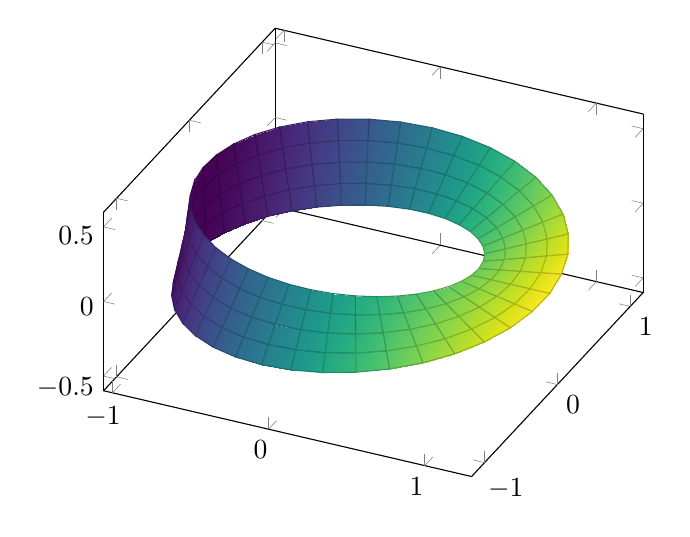
\begin{tikzpicture}
            \centering
            \begin{axis}[
                unit vector ratio=1 1 1
            ]
                \addplot3 [
                    surf, shader=faceted interp,
                    point meta=x,
                    colormap/viridis,
                    samples=40,
                    samples y=5,
                    z buffer=sort,
                    domain=0:360,
                    y domain=-0.5:0.5
                ] (
                    {(1+0.5*y*cos(x/2))*cos(x)},
                    {(1+0.5*y*cos(x/2))*sin(x)},
                    {0.5*y*sin(x/2)});
            \end{axis}
        \end{tikzpicture}
    \caption{M\"obius surface}
    \label{fig:mobius}
    \end{figure}
\end{exmp}

\begin{rmk}
    Given a local parameterization $m: U \subseteq \R^2 \to S$, then one unit normal vector at $p \in m(U)$ is given by
    \begin{align*}
        N(p) = \frac{m_u \times m_v}{\norm{m_u \times m_v}},
    \end{align*}
    where $m_u$ and $m_v$ are the partials derivatives of $m$. Note that $-N(p)$ is also a unit normal vector $p$. Since $TpS$ is independent of any local parameterization, so is $\pm N(p)$ (up to sign). Furthermore, since charts are smooth, so is the unit normal.
\end{rmk}

\begin{thm}\label{thm:orientable-atlas}
    A regular surface $S$ is orientable if and only if there exists an atlas $\{m_i: U_i \subseteq \R^n \to S\}$ such that for any $m_i(u_i, v_i), m_j(u_j, v_j)$, the transition map
    \begin{align*}
        \frac{\partial (u_i, v_i)}{\partial (u_,v_j)} = \begin{pmatrix}
            \frac{\partial u_i}{\partial u_j} & \frac{\partial u_i}{\partial v_j} \\
            \frac{\partial v_i}{\partial u_j} & \frac{\partial v_i}{\partial v_j}
        \end{pmatrix}
    \end{align*}
    has positive determinant at all $p \in m_i(U_i) \intersect m_j(U_j)$.
\end{thm}

\begin{proof}
    If $m: U \to S$ and $w: V \to S$ are two local parameterizations such that $p \in m(U) \intersect w(V)$, then $m_u \times m_v = \frac{\partial (u,v)}{\partial (a, b)}(w_a \times w_b)$. Therefore, the unit normals defined by distinct overlapping charts are the same if and only if the transition map has strictly positive determinant.
\end{proof}

\begin{cor}
    If a surface has a global parameterization, then it is orientable.
\end{cor}

\begin{prop}
    If a regular surface $S$ can be covered by two charts $m: U \to S$ and $w: V \to S$ such that $m(U) \intersect w(V)$ is connected, then $S$ is orientable.
\end{prop}

\begin{proof}
    The determinant of the transition map is continuous and non-zero, so it must be positive on all of $m(U) \intersect w(V)$, or negative on all of $m(U) \intersect w(V)$. If it is positive, then by Theorem \ref{thm:orientable-atlas} we are done. Otherwise, we replace the chart $w$ with $q(u, v) = w(u, v)$. Then $q$ is still a chart, with the same image (although a different domain), but the rows of the transition map are swapped, and therefore the determinant of the transition map is now positive.
\end{proof}

\begin{prop}
    Let $S$ be a regular surface defined by $S = f^{-1}(\{a\})$ for some $f: \R^3 \to \R$, where $f$ is smooth and $a$ is a regular value of $f$. Then $S$ is orientable.
\end{prop}

\begin{proof}
    Since $\nabla f(p)$ doesn't vanish on $S$, we know that $\nabla f(p)/\norm{\nabla f(p)}$ defines a unit normal for all $p \in S$. Since $f$ is smooth, so is $\nabla f$, and so this unit normal vector field is smooth.
\end{proof}

\section{Gauss map}

\begin{defn}
    Let $S$ be an orientable surface. A smooth unit normal vector field $N$ on $S$ is the \emph{orientation}
\end{defn}

\begin{defn}
    Let $S$ be a regular surface with orientation $N$. We define the \emph{Gauss map} from $\R^3 \to \R^3$ as $p \mapsto N'(p)$.
\end{defn}
